\documentclass{article}

%----------------------------------------
% Packages
%----------------------------------------
\usepackage{booktabs}
\usepackage[algo2e]{algorithm2e}
\usepackage[left=1in, right=1in, top=1in, bottom=1in]{geometry}
\usepackage{graphicx}
\usepackage{amsmath,amsbsy,amssymb,amsfonts,amsthm}
\usepackage{nicefrac}
\usepackage{mathtools}
\usepackage{color}
\usepackage{xspace} % Correct macro spacing
\usepackage[numbers]{natbib} % For citations
\usepackage{times}
\usepackage{graphicx,subfigure}
%\usepackage[small,bf]{caption}
\usepackage{algorithm,algorithmic} 
\usepackage{hyperref}
\usepackage{url}

\usepackage{xcolor}
\usepackage{shadethm}

\usepackage{fancyhdr}
\pagestyle{fancy}
\lhead{This is my name}
\rhead{this is page \thepage}

\usepackage{fancyhdr}
\pagestyle{fancy}
\lhead{IFT 6085 - Theoretical principles for deep learning}
\rhead{Lecture 6: January 23, 2020}


\newshadetheorem{thm}{Theorem}
\newshadetheorem{defn}[thm]{Definition}
\newshadetheorem{assm}[thm]{Assumption}
\newshadetheorem{prop}[thm]{Property}
\newshadetheorem{eg}[thm]{Example}



\usepackage{tikz}
% Optional PGF libraries
\usetikzlibrary{shapes,snakes}
\usepackage{pgf}
\usepackage{pgflibraryarrows}
\usepackage{pgflibrarysnakes}
\usetikzlibrary{decorations.text}
\usepgfmodule{shapes}
%\usetikzlibrary{arrows}
\usetikzlibrary{decorations.pathmorphing}
\usetikzlibrary{decorations.markings}
\usetikzlibrary{patterns}
\usetikzlibrary{automata}
\usetikzlibrary{positioning}
%\usepackage{tikz-cd}
\usepackage{pgfplots}
%\usepackage{tkz-euclide}
%\usetkzobj{all}
\usetikzlibrary{backgrounds}
%\usetikzlibrary{fillbetween,backgrounds}



\tikzset{->-/.style={decoration={
 markings,
 mark=at position #1 with {\arrow{>}}},postaction={decorate}}}
 
 \tikzset{cross/.style={cross out, draw=black, minimum size=5, inner sep=0pt, outer sep=0pt},
%default radius will be 1pt. 
cross/.default={1pt}}

\tikzset{->-/.style={decoration={
 markings,
 mark=at position #1 with {\arrow{>}}},postaction={decorate}}}


\definecolor{shadethmcolor}{HTML}{F0F0F0}
%\definecolor{shadethmcolor}{HTML}{EDEDED}
%\definecolor{shadethmcolor}{HTML}{EDF8FF}
%\definecolor{shaderulecolor}{HTML}{EDF8FF}
%\definecolor{shaderulecolor}{HTML}{45CFFF}
\setlength{\shadeboxrule}{.4pt}


\setlength\parindent{0pt}

% Packages hyperref and algorithmic misbehave sometimes.  We can fix
% this with the following command.
\newcommand{\theHalgorithm}{\arabic{algorithm}}

%----------------------------------------
% Standard macros
%----------------------------------------


%----------------------------------------
% Project-specific macros
%----------------------------------------

%----------------------------------------
% Header
%----------------------------------------
\title{IFT 6085 - Lecture 6 \\ 
Nesterov's Momentum, Stochastic Gradient Descent }
\date{}

%----------------------------------------
% Document
%----------------------------------------
\begin{document} 

%----------------------------------------
% Abstract
%----------------------------------------
\maketitle


\vspace{-0.5in}
\begin{center}
This version of the notes has not yet been thoroughly checked.
Please report any bugs to the scribes or instructor.
\end{center}
\vspace{0.2in}

\textbf{Scribes:}\hfill
\textbf{Instructor:}  Ioannis Mitliagkas\\
\textbf{Winter 2020:} Manuela Girotti\\
\textbf{Winter 2019:} Yann Bouteiller \& Remi Piche-Taillefer\\
\textbf{Winter 2018:} Charles Ashby \& Gabriele Prato


%----------------------------------------
% Body
%----------------------------------------

\newcommand{\infgc}{\inf_{g \in \mathcal{C}}}
\newcommand{\supgc}{\sup_{g \in \mathcal{C}}}

\newcommand{\Prob}{\mathbb{P}}
\newcommand{\E}{\mathbb{E}}
\newcommand{\reals}{\mathbb{R}}

\newtheorem{note}[thm]{Remark}
\newshadetheorem{lemma}[thm]{Lemma}

\def\R{\mathbb{R}}
\def\le{\left}
\def\ri{\right}




\section{Summary}

This lecture covers the following elements of optimization theory:

\begin{itemize}
\item Failing case of Polyak's momentum
\item Nesterov's momentum
\item Stochastic gradient descent
\end{itemize}
Most of the lecture has been adapted from \cite{2015arXiv1405.4980v2}, \cite{2014arXiv1408.3595L}, \cite{Nesterov1998} and \cite{Shalev2014}.

\section{Failing case of Polyak's Momentum}
In the previous lecture we presented Polyak's momentum algorithm (or heavy-ball method), in which the iteration step is given by:
\begin{equation} \label{eq:1}
	x_{t+1} = x_t - \alpha \nabla f(x_t) + \beta (x_t - x_{t-1}), \quad  \alpha > 0, \beta \in [0,1]
\end{equation}

This method is known to be robust and effective in many real-world applications. However, in a paper published in 2015, \citet{2014arXiv1408.3595L} have shown that there exist strongly-convex and smooth functions for which, by choosing carefully the hyperparameters $\alpha$ and $\beta$ and the initial condition $x_0$, the heavy-ball method fails to converge. We give here merely the intuition behind the malfunction of the algorithm as well as empirical results taken from the paper.

\vspace{2ex}

% Consider the following function:\\% \citet{2014arXiv1408.3595L} give the following one-dimensional example :\\
Let $f$ be a piece-wise quadratic function whose gradient is:
\begin{gather}
	\nabla f(x) =  \begin{cases}
    25x &   x < 1 \\
    x+24   &  1 \leq x < 2 \\
    25x-24 & x \geq 2
\end{cases}
\end{gather}
By construction,  $\forall \ x_1, x_2, \|\nabla f(x_1)-\nabla f(x_2)\| \leq 25\|x_1 - x_2\|$, therefore $f$ is $25$-smooth, and 
%. Let us note the following quantities : 
%$$
%\nabla (f(x) - \frac{\|x\|^2}{2}) = \nabla f(x) - x = 
%\begin{cases}
%    24x & \text{if }  x < 1 \\
%    24   & \text{if } 1 \leq x < 2 \\
%    24x-24 & \text{otherwise} 
%\end{cases}
%$$
%$$
%\nabla^2 (f(x) - \frac{\|x\|^2}{2}) =
%\begin{cases}
%    24 & \text{if }  x < 1 \\
%    0   & \text{if } 1 \leq x < 2 \\
%    24 & \text{otherwise} 
%\end{cases}
%$$
\begin{gather}
\nabla^2 f(x) =
\begin{cases}
    25 &  x < 1 \\
    1   &  \leq x < 2 \\
    25 & x\geq 2
\end{cases}
\end{gather}
implying $\nabla^2 f \geq 1>0$, therefore $f$ is 1-strongly convex.\\

In \figurename \ \ref{iteratesPolyak} are displayed the first 50 iterates of Polyak's momentum algorithm applied to $f$, using $\alpha=\frac{1}{9}$, $\beta=\frac{4}{9}$ and $x_0=3.3$. The output values are bound to cycle through 3 points indefinitely.

\begin{figure}
  \centering
   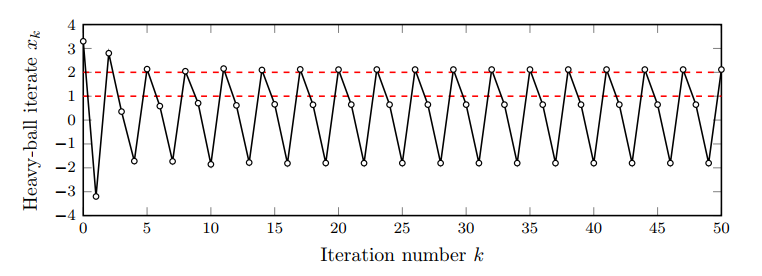
\includegraphics[width=15cm, height=4cm]{images/iterates.png}
  \caption{Value of $x_k$ for the 50 first iterations of Polyak's momentum algorithm. The dashed red lines separate the pieces of $f(x)$. Taken from \citet{2014arXiv1408.3595L}. \label{iteratesPolyak} }
  \label{figIt}
\end{figure}

We can see that despite the function $f$ being 1-strongly convex and 25-smooth, the Polyak's GD map $\Phi_{P-GD}$ has a periodic point of period 3 and its flow is an attractive limit-cycle (see the proof in \cite{2014arXiv1408.3595L}, Appendix B).
%Despite the fact that $f$ is 1-strongly convex and 25-smooth, Polyak's momentum algorithm loops indefinitely over these points. \citet{2014arXiv1408.3595L}'s proof revolves around the idea that the iterates are stuck in a limit cycle. 
%The authors show that the following sub-series of the iterates tend to three points that are not the optimal value of $f$.
In particular, the authors in  \cite{2014arXiv1408.3595L} show that with the parameters $\alpha$ and $\beta$ given as in \figurename \ \ref{iteratesPolyak}, there exists a sequence of iterates $\{x_t\}$ such that as $n\to \infty$
\[
	x_{t=3n} \rightarrow p \approx 0.65, \quad x_{t=3n+1} \rightarrow q  \approx -1.80, \quad x_{t=3n+2} \rightarrow r \approx 2.12.
\]
See \figurename \ \ref{plot3cycle} for  a visalization of the effect of the map $\Phi_{P-GD}$ on the cycle $\{p,q,r\}$.

\begin{figure}[h]
  \centering
  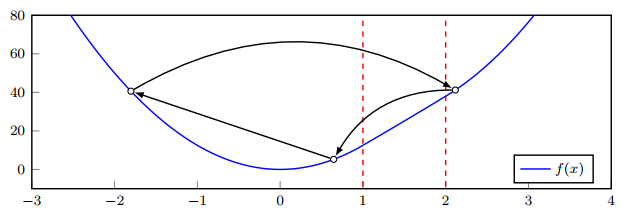
\includegraphics[scale=0.5]{images/plot_f.png}
  \caption{Illustration of the limit values of the failing case of Polyak's momentum algorithm, the dashed red lines separate the pieces of $f$. Image taken from \citet{2014arXiv1408.3595L}. \label{plot3cycle}}
\end{figure}


\subsection{Food for thought}
The result shown in \cite{2014arXiv1408.3595L} is certainly helpful in understanding the powerfulness and the limitations of Polyak's algorithm. However, it is worth pointing out that Polyak's momentum GD has guaranteed convergence for quadratic functions (and not piece-wise quadratic). \\

%In an attempt to resize the implications of Lessard's counterexample, we can state that the authors in \cite{2014arXiv1408.3595L} showed that for a methodically tuned case and for a restricted range of initial condition $x_0$, Polyak's momentum algorithm does not converge to the minimizer of the function under exam. \\

Let us look at it from a broader perspective. Consider the family of continuous functions $\{f_{\omega,\epsilon}\}$ with gradient
\begin{gather}
	\nabla f_{\omega, \epsilon}(x) =  \begin{cases}
    25x &   x < 1 \\
    \omega x+24   &  1 \leq x < 1+\epsilon \\
    25x-24 & x \geq \epsilon
\end{cases}
\end{gather}
This is a set of piece-wise continuous and piece-wise quadratic functions, where $\omega >0$ represents the curvature of the function within a (small) window of size $\epsilon \geq0$. The counterexample from \cite{2014arXiv1408.3595L} falls into this set with $\omega =\epsilon = 1$.\\

By construction, each function in this family is $\alpha$-strongly convex and $25$-Lipschitz (let's assume $\omega <25$): therefore its condition number is $\kappa = \frac{25}{\omega}$, which can be arbitrarily high for very small values of $\omega$. 

On the other hand, $\forall \ \omega>0$ fixed, $f_{\omega, \epsilon} \to f_0$ uniformly, where $f_0$ is the corresponding quadratic function with window-size $\epsilon =0$, which clearly has condition number $\kappa = 1$.\\

Considering the Polyak's algorithm on this family of functions and their limit, we have optimal tuning for $f_0$ with step size $\alpha = \frac{1}{25}$ and momentum $\beta = 0$, while for $f_{\omega,\epsilon}$ the optimal tuning gives a value for the momentum 
$$\beta = \le(\dfrac{\sqrt{\kappa} -1}{\sqrt{\kappa}+1}\ri)^2 \approx 1 \qquad \text{for large values of } \omega.$$

This mismatch between condition numbers of $\{f_{\omega,\epsilon}\}$ and their limit $f_0$, while a uniform convergence result holds, may suggest that for some families of functions Polyak's tuning is problematic. Otherwise said: there could be a better strategy for tuning the step size and the momentum parameter that can still yield convergence; finally, the quest for a better tuning could require a new innovative definition of condition number that would allow to extend convergence results to functions that are not simply quadratic. 
Indeed, numerical evidence shows that Polyak's momentum has still a lot of potential to be successfully applied to a broad class of functions.


%Many questions remains open: is the set of strongly convex, Lipschitz function for which Polyaks' momentum does not work consistently big? (this would require embedding a measure on this set ....)
%
%
%Much richer zoo of functions 
%subfamilies of stringly-convex, lipschitz functions for which it works


\section{Nesterov's Accelerated Gradient Descent}

\subsection{Motivation}

In the last section, we saw that Polyak's momentum algorithm can fail to converge for some carefully built convex optimization problems. Leveraging the idea of momentum introduced by Polyak, Nesterov introduced a slightly altered update rule that has been shown to converge not only for quadratic functions, but for general convex functions. 
%Despite extending the hypothesis space for $f$, this algorithm still manages to achieve an acceleration rate comparable to the heavy-ball method. 
The main ideas of this demonstration are presented at the end of this section.\\

The Nesterov's Accelerated Gradient algorithm is described as follow by \citet{Sutskever2013}:
\begin{algorithm}[H]
\SetAlgoLined
\textbf{parameters:} number of iterations $T$, step size $\alpha$, momentum $\beta$ and initial condition $x_0$.

\textbf{initialize:} $v_0 \gets 0$

\For{$t=0,\ldots, T-1$}{
  $v_{t+1} \gets \beta v_t - \alpha \nabla f(x_t + \beta v_{t})$\;
  
  $x_{t+1} \gets x_{t} + v_{t+1}$\;
  
 }
 
 \textbf{return } $x_{T}$
 \caption{Nesterov's Accelerated Gradient Descent \label{NAGD}}
\end{algorithm}

% Note: Despite being slightly different from the formulation seen in class, this writing makes it much easier to see what's going on. It is taken directly from "On the importance of initialization and momentum in deep learning""

The quantity $v_{t+1}$ can be thought of as the velocity at time $t$ or as the displacement vector: it is calculated by applying the  momentum $\beta$ to the previous $v_t$ displacement and subtracting the gradient step to $x_t + \beta v_t$, which is the point where the momentum term leads from $x_t$. 
Rewriting these two sequences as one yields:
\begin{equation} \label{eq:2}
	x_{t+1} = x_t + \beta(x_t - x_{t-1}) - \alpha \nabla f(x_t + \beta (x_t - x_{t-1}))
\end{equation}

Comparing equation \eqref{eq:1} with equation \eqref{eq:2}, we can see that Polyak's method evaluates the gradient before adding momentum, whereas Nesterov's algorithm evaluates it after applying momentum, which intuitively brings us closer to the minimum $x^*$, as illustrated in \figurename \ \ref{fig:momentum_comparison}.

\begin{figure}[H]
  \centering
  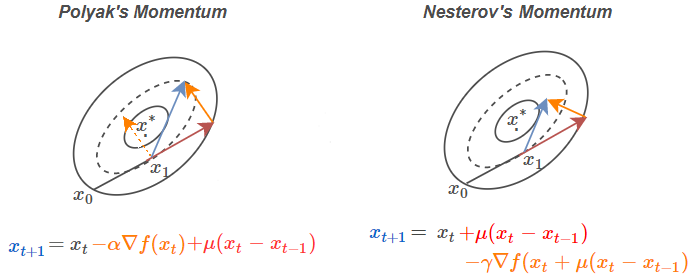
\includegraphics[width=0.8\textwidth]{images/polyak_diff1.PNG}
  \caption{Comparison between Polyak's and Nesterov's momentum. The gradient descent step (orange arrow) is perpendicular to the level set before applying momentum to $x_1$ (red arrow) in Polyak's algorithm, whereas it is perpendicular to the level set after applying momentum to $x_1$ in Nesterov's algorithm.}
  \label{fig:momentum_comparison}
\end{figure}

The convergence rate (upper bound on the sub-optimality) for different classes of functions for gradient descent and Nesterov's accelerated gradient descent are compared in Table \ref{labt1}.

\begin{table}[H]
  \caption{Convergence rate for Gradient Descent \& Nesterov's Accelerated Gradient}
  \label{sample-table}
  \centering
  \begin{tabular}{lll}
   \\
    Class of Function & GD & NAG  \\
    \midrule
    Smooth & $\mathcal O(1/T)$ & $ \mathcal O(1/T^2)$   \\
    Smooth \& Strongly-Convex & $ \mathcal O\left(exp \left(-\frac{T}{\kappa}\right)\right)$  & $ \mathcal O\left(exp \left(-\frac{T}{\sqrt[]{\kappa}}\right)\right)$\\
    \bottomrule
  \end{tabular}
  \label{labt1}
\end{table}

Nesterov's Augmented Gradient in the case of smooth and strongly convex functions gives the acceleration that we had with Polyak's momentum for quadratic functions. This is great, because we get the guarantee for a more general class of functions. Recall that if $f$ is $\mu$-strongly convex and $\lambda$-smooth then $\kappa = \frac{\lambda}{\mu}$. Therefore, when $\lambda << \mu$ (i.e. some dimensions have very steep gradients), the acceleration becomes very significant.
\newline

\subsection{General scheme for the Convergence of Nesterov's Accelerated Gradient Descent}
In this section, we present the main items behind the proof of convergence for Nesterov's momentum algorithm for general convex functions. In order to achieve this proof, Nesterov uses an \textbf{estimate sequence}.

\begin{defn}[Estimate Sequence; \cite{Nesterov1998}, Definition 2.2.1]
A pair of sequences $\left\{ \phi_k(x) \right\}_{k=0}^\infty$ and $\left\{ \lambda_k \right\}_{k=0}^\infty$ where $\lambda_k \geq 0$, is called an Estimate Sequence of $f$ if the following conditions hold:
\begin{itemize}
\item $\lambda_k \mathop{\to} 0$ when $k \to \infty$
\item $\forall \ x \in \mathbb{R}^n, \forall \ k \geq 0$, the following holds: 
\[
\phi_k(x) \leq (1- \lambda_k) f(x) + \lambda_k \phi_0 (x)
\]
\end{itemize}
\label{defEstim}
\end{defn}

\figurename \ \ref{figEstim} illustrates the way an estimate sequence aligns with the $f$ function. The Definition above is suggesting that an estimate sequence has the property that the functions $\{\phi_k\}$ are pointwise ``not too far above" the function $f$ itself, for each $k\in \mathbb{N}$: 
$$ \phi_k(x) \leq f(x) + \lambda_k\le( \phi_0 (x)-f(x) \ri), $$
since $\lambda_k \to 0$ and we can assume that the function $f$ and $\phi_0$ are sufficiently regular so that the difference $ \phi_0 (x)-f(x)$ is bounded in norm (at least pointwise). It also follows easily that $\forall \ x \in \mathbb{R}^n$
\begin{equation} \lim_{k\to\infty}{\phi_k(x)} \leq f(x),
\end{equation}
therefore, in the limit as $k \to \infty$, $\phi_k$ becomes a lower bound of $f$. \\
%, since $\lambda_k \phi_0 (x) \to 0$ and $(1- \lambda_k) f(x) \to f(x)$.


\begin{figure}
  \centering
  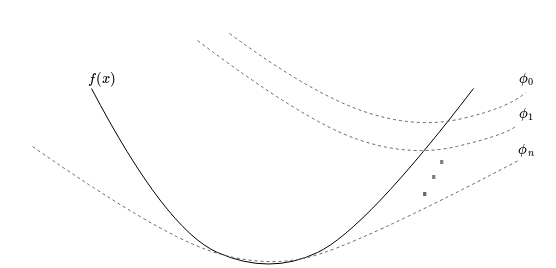
\includegraphics[width=10cm]{images/estimate_sequence1.png}
  \caption{Example of an estimate sequence}
  \label{figEstim}
\end{figure}


Although the definition of estimate sequence sounds extremely artificial and lacking intuition, Nesterov showed that provided we manage to find such a sequence, then there is an automatic way to construct a sequence of iterates $\{x_k\}$ that successfully converges to the minimizer $x^\ast$ with rate of convergence given by the rate of convergence of the sequence of $\{\lambda_k\}$ to 0.\\

Let us start with formalizing the last claim:

%The idea is to find an estimate sequence $\phi$ to help us minimize $f$. To do so, the author introduces the following result:

\begin{thm}[\cite{Nesterov1998}, Theorem 2.2.1]\label{Thm221}

Given a $\mu$-strongly convex, $L$-smooth function $f$ on $\R^n$, an estimate sequence $\le( \{\phi_k(x)\}_{k=0}^\infty, \{\lambda_k\}_{k=0}^\infty \ri)$ of $f$ and a corresponding sequence of iterates $\{x_k\}$ such that 
$$f(x_k) \leq \phi_{k}^{\ast} =: \min\limits_{x} \phi_k (x), \qquad \forall \ k \in \mathbb{N},$$ 
then
\[
	f(x_k) - f(x^*) \leq \lambda_k \left[ \phi_0(x^*) - f(x^*) \right].
\]
\end{thm}
%Since $\phi_0(x^*) - f(x^*)$ is a fixed quantity, the rate of convergence for the sub-optimality will depend on how quickly $\lambda_k$ decreases to 0. 

Therefore, provided that 
\figurename \ \ref{Thm221plot} presents a visualization of Theorem \ref{Thm221}. 
\begin{figure}
  \centering
  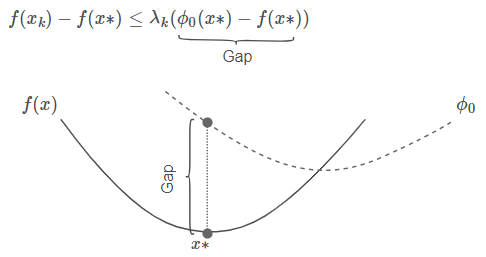
\includegraphics[width=10cm]{images/gap1.PNG}
  \caption{Illustration of Theorem \ref{Thm221}.\label{Thm221plot}}
\end{figure}
\newline


In \cite{Nesterov1998} (Lemma 2.2.2 and Lemma 2.2.3), Nesterov already provided us with a recipe for an estimate sequence for a generic $\mu$-strongly convex, $L$-smooth function $f$: 
\begin{enumerate}
\item Pick a starting point $x_0$;
\item Set  $\lambda_0 = 1$, $\phi_0{(x)} = f(x_0) + \frac{\mu}{2}\|{x - x_0}\|^2$.
\item Define recursively the rest of the sequence as
\begin{align}
& \lambda_{k+1} = (1-\alpha_k)\lambda_k, \\
& \phi_{k+1}(x) = (1-\alpha_k)\phi_k(x) + \alpha_k\left( f(y_k) + \langle\nabla f(y_k), x-y_k\rangle + \frac{\mu}{2}\lVert{x - y_k}\rVert^2\right ) ,
\end{align}
where $\{y_k\}_{k=0}^{\infty} \subseteq \R^n$ and  $\{\alpha_k\}_{k=0}^{\infty} \subseteq \R$ are two arbitrary control sequences (as of now we only require $\{\alpha_k\}_{k=0}^{\infty}$ to be such that such that $\alpha_k \in (0, 1)$ and $\sum_{k=0}^\infty{\alpha_k} = +\infty$). 

Note that by construction, the family of functions $\{\phi_k\}$ have all the same curvature $\mu$.
\end{enumerate}



We can think of $\{y_k\}$ and $\{\alpha_k\}$ as a set of parameters that we can smartly pick (with tears; see \cite{Nesterov1998}, General Scheme 2.2.6) in order to guarantee that 
\begin{gather}
\text{for each iteration step } k \in \mathbb{N}, \ \exists \ x_k \in \R^n: \quad f(x^\ast) \leq f(x_k) \leq  \min\limits_{x} \phi_k (x) =: \phi_k^\ast\label{eq11}
\end{gather}

Note that only the value of the function at the iterate $x_k$ is bounded above by $\phi_k$, not the entire function $f$. 
%The intuition behind \eqref{eq11} is that since $\{\phi_k\}$ is part of an estimate sequence, we know that
%\begin{itemize}
%\item by definition, for each $k$, the function $\phi_k$ is ``not too far from" $f$ \underline{for all} values of $x \in \R^n$ and the distance from $f$ diminishes as $k$ increases (we have an explicit control over this distance);
%\item in the limit as $k \to +\infty$, the sequence becomes a lower bound of $f$ over the whole domain  $\forall \ x \in \R^n$;
%\end{itemize} 
%Given these properties, \eqref{eq11} assures that at each iteration $k$,  $f(x^\ast) \leq f(x_k ) \leq \phi_k^\ast$ and 
Finally, $\phi_k$ becomes an increasingly good upper bound and although we lost the relaxation property on $f$ (Nesterov's algorithm has momentum), the sequence $\{\phi_k^\ast\}$ is decreasing and forces the iterates $\{x_k\}$ to converge towards the minimizer $x^\ast$.
% (in fact, it is possible to prove that it decreases geometrically towards the minimum of $f$). 


%This carefully designed sequence is then used to show how $\lambda_k$ can converge efficiently, and how the minimum point of $\phi_k$ converges to $x^*$.



\section{Stochastic Gradient Descent}

\subsection{Motivation}

As we have seen in the previous lecture, Gradient Descent (GD) is not subject to variance since at every step we compute the average gradient using the whole dataset. The downside is that every step is very computationally expensive, $\mathcal O(nd)$ per iteration, where $n$ is the number of samples in our dataset and $d$ is the number of dimensions of $x$. Since we need $\mathcal O(d)$ iterations to converge, the total problem cost is about $\mathcal O(nd^2)$.\\

GD becomes impractical when dealing with large datasets. This is where Stochastic Gradient Descent (SGD) comes in. It is a modified version of GD which does not use the whole set of examples to compute the gradient at every step. 
In SGD we allow the direction towards which want to update the (weight) parameter ${\bf w}$ to be a random vector as long as its expected value at each iteration will equal the gradient.% (or, more generally, a subgradient of the function at the current vector). %It is a \underline{random} algorithm. 

By doing so, we can reduce computation all the way down to $\mathcal O(d)$ per iteration, instead of $\mathcal O(nd)$. \\



We consider a large class of functions for which SGD performs well, in particular we will not require the function $f$ that we want to minimize to be differentiable (hence, the need of a ``subgradient" $\partial f$, see Definition \ref{subgraddefn}). 

Let $f: \R^n \to \R$, $f =f({\bf w})$:
%\begin{algorithm}[H]
%\SetAlgoLined
%\textbf{Require:} training time T, learning rate $\gamma$, batch size $K$ and parameter's initialization $x_0$.
%
%\For{$t\gets0$ \KwTo $T-1$}{
%  Sample $(i_1, ..., i_K) \sim U^{K} (1, ..., n)$\;
%  
%  $x_{t+1} = x_{t} - \gamma \frac{1}{K} \sum_{j=1}^{K} \nabla f_{i_j}(x_t)$\;
%  
% }
% 
% \textbf{return } $x_{T-1}$
% \caption{Stochastic Gradient Descent }
%\end{algorithm}
\begin{algorithm}[H]
\SetAlgoLined
\textbf{parameters:} number of iterations T, step size $\eta$ %, batch size $K$ and parameter's initialization $x_0$.

\textbf{initialize:} ${\bf w}^{(1)} \gets {\bf 0}$

\For{$t=1,2,\ldots T$}{
  choose ${\bf v}_t$ at random from a distribution such that $\E[{\bf v}_t | {\bf w}^{(t)}] \in \partial f ({\bf w}^{(t)})$
  
  update ${\bf w}^{(t+1)} \gets {\bf w}^{(t)} - \eta {\bf v}_t$
 
 }
 
 \textbf{output} $\bar{\bf w} = \frac{1}{T} \sum_{t=1}^T {\bf w}^{(t)}$
 \caption{Stochastic Gradient Descent \label{SGDalgo}}
\end{algorithm}


\begin{note}
It is important to stress that in general each random vector ${\bf v}_t$ is dependent on the previously generated vectors $\{{\bf v}_1, \ldots, {\bf v}_{t-1} \}$.
\end{note}

%\begin{note}
The strategy to (randomly) choose the vector ${\bf v}_t$ could vary depending on the applications. In the ML world, we want to minimize the empirical risk (ERM method)
$$J({\bf w}) = \dfrac{1}{n} \sum_{i=1}^n \ell(f_{{\bf w}}(x_i),y_i),$$
where $\{(x_1,y_1), \ldots, (x_n,y_n)\}$ is the collection of (labelled) samples drawn from an unknown distribution, $f_{\bf w}$ is the predictor, $\ell$ is the loss function (we assume them to be differentiable).

\vspace{2ex}

In this setting, SGD is set up in the following way: at every iteration $t$ of the optimization method, we randomly draw an index $i_t$ uniformly among the set of indices $\{1, \ldots, n\}$: $i_t \sim U(\{1, \ldots, n\})$. We then perform GD on the function $\ell(f_{\bf w}(x_{i_t}),y_{i_t})$, i.e. we set ${\bf v}_t = \nabla \ell (f_{\bf w}(x_{i_t}),y_{i_t}) $
and we perform the weight update ${\bf w}^{(t+1)} = {\bf w}^{(t)} -\eta {\bf v}_t.$
%\end{note}
\\


Note that in expectation, the convergence is equivalent to GD, since $\mathop{\mathbb{E}}_{i_t \sim U(\{1, ..., n\})} \left [{\bf v}_{t} \right ] = \nabla J({\bf w})$, therefore, the expected iterate of SGD converges to the optimum. The downside is that stochasticity brings variance. Even if SGD is shown to converge, the variance can seriously handicap the convergence rate as we will see in Subsection \ref{BVtradeoff}. This is especially true the smaller the batch size is, as variance is inversely proportional to the number of examples used to compute the gradient at every step.\\

SGD's convergence rate for Lipschitz, convex functions is $\mathcal{O}(T^{-1/2})$, as we will see in Subsection \ref{SGDbound}, and $\mathcal{O}(T^{-1})$ for strongly convex. More iterations are needed to reach the same accuracy as GD, but the iterations are far cheaper.

\subsection{Bias-Variance Trade-off}\label{BVtradeoff}

Recall from the last lecture that the iteration step at time $t$ for Gradient Descent is given by $x_{t+1} = x_{t} - \gamma \nabla f(x_t)$ where $\nabla f(x) = \frac{1}{n}\sum_{i=1}^{n}f_i(x)$. The variance from SGD comes from the fact that we do not take the average gradient over the whole dataset.\\

When training begins, the model weights $x$ are more than likely very far from the optimal value $x*= \min_{x}f(x)$, therefore, most of our data points $x_i$, agree on the direction of the gradient. (see the high bias region in Figure 6)\\

However, when training goes on, most of the model weights are already close to the optimum, some are well tuned and others are not, this is where the variance has a significant impact on our convergence rate because almost all samples in our batch will produce gradients pointing in different directions, therefore, if we keep the same step size we will bounce around the optimum. This is called the noise ball effect.\\

To avoid bouncing around the minimum, we can use a decaying step size. The blue line in Figure 6 illustrates what happens when we reduce the variance by decaying the step size, another trick to reduce the variance would be to increase the batch size (in the limit we would get the same convergence rate as Gradient Descent).

\begin{figure}[H]
  \centering
  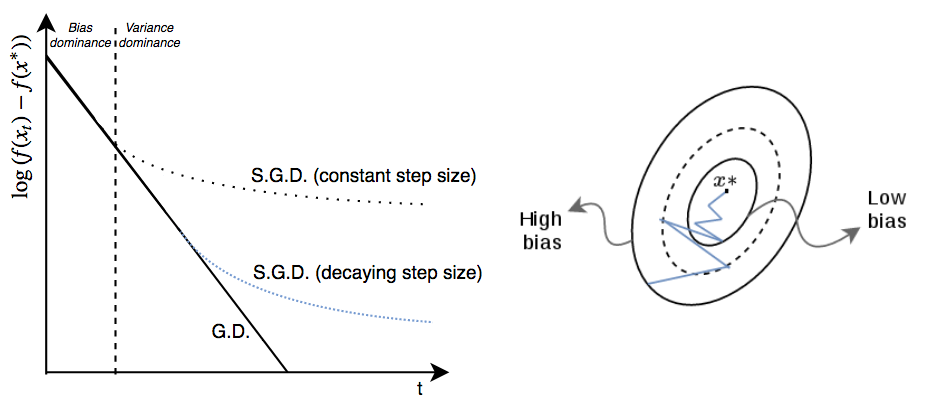
\includegraphics[width=0.7\textwidth]{images/gd_sgd_convergence.PNG}
  \caption{Convergence for Gradient Descent and Stochastic Gradient Descent. The blue line on the left plot illustrates what happens when we decay the step size. The red line shows what happens with constant step size, notice how it flattens out on the left plot.}
\end{figure}


\subsection{Convergence rate for convex-Lipschitz-bounded functions}\label{SGDbound}


We provide here an upper bound on the suboptimality of the solution obtained with SGD with respect to the minimizer ${\bf w}^\ast$. Similar to the case of GD (see Theorem 1 from Lecture 2 of the course), we can show that SGD has convergence rate of the order of $\mathcal{O}(T^{-1/2})$ for convex, $L$-Lipschitz functions, where $T$ is the number of iterates. However, since SGD is a random algorithm, we can only give this result in ``expected" form. \\


Before stating the theorem, which will be valid for general non-differentiable, convex, Lipschitz function, we quickly recall the definition of the subgradient: the subgradient is a generalization of the gradient for non-differentiable functions. Similar to the gradient, a subgradient of a function $f$ at a point ${\bf x}$ is the slope of a tangent line that bounds the function $f$ at the point ${\bf x}$ from below. See \figurename \ \ref{subgrad}. \\
\begin{defn}\label{subgraddefn}
Given a convex function $f:S\to\R$, with $S \subseteq \R^n$ a convex set, a vector ${\bf v} \in R^n$ is a {\bf subgradient} of $f$ at the point ${\bf x}$ if
$$ f({\bf y}) \geq f({\bf x}) + \langle {\bf y} - {\bf x}, {\bf v} \rangle, \qquad \forall \ {\bf y} \in S.$$
The set of all subgradients of $f$ at the point ${\bf x}$ is called {\bf differential set} and it is denoted $\partial f ({\bf x})$.
\end{defn}
It is clear that in case of differentiable functions the subgradient consists of only one element, which is indeed the gradient of the function ( $\partial f ({\bf x}) = \{ \nabla f({\bf x})\} $).\\






\begin{figure}
\centering
\begin{tikzpicture}[>=stealth, scale=1]

\draw[->] (-1,0) -- (4,0) node[right] {$\R^n$};
\draw[->] (-0.5,-0.5) -- (-.5,4) node[above] {$\R$};
\draw[domain=0.25:3.75,smooth,variable=\x,blue, thick] plot ({\x},{(\x-2)^2+1});


\node[below] at (1.5,0) {${\bf x}$};
\draw[fill] (1.5,0) circle [radius=0.05];

\node[below] at (.5,0) {${\bf y}$};
\draw[fill] (.5,0) circle [radius=0.05];


\node[above right] at (1.5,5/4) {$f({\bf x})$};
\draw[fill] (1.5,5/4) circle [radius=0.05];

\node[above right] at (0.5,3.25) {$f({\bf y})$};
\draw[fill] (0.5,3.25) circle [radius=0.05];
\draw[fill] (0.5,2.25) circle [radius=0.05];

\draw[dashed,thick] (-.5,3.25) -- (11/4,0) node[midway,sloped,below] {$f({\bf x}) + \langle {\bf y}- {\bf x}, \nabla f({\bf x}) \rangle$};;

\end{tikzpicture}
\qquad
\begin{tikzpicture}[>=stealth, scale=1]

\draw[->] (-1,0) -- (4,0) node[right] {$\R^n$};
\draw[->] (-0.5,-0.5) -- (-.5,4) node[above] {$\R$};
\draw[domain=1.5:3.75,smooth,variable=\x,blue, thick] plot ({\x},{3/2*\x- 1});
\draw[domain=-0.5:1.5,smooth,variable=\x,blue, thick] plot ({\x},{-3/2*\x+14/4});



\node[below] at (1.5,0) {${\bf x}$};
\draw[fill] (1.5,0) circle [radius=0.05];



\node[above] at (1.5,1.75) {$f({\bf x})$};
\draw[fill] (1.5,5/4) circle [radius=0.05];

%\draw[dashed,thick] (-.5,3.25) -- (11/4,0) ;
\draw[dashed,thick] (-.5,5/4) -- (4,5/4) ;
\draw[dashed,thick] (-.5,-5/12) -- (4,10/3) ;
\draw[dashed,thick] (-.5,2) -- (4,0.3125) ;

\end{tikzpicture}
\caption{Left: for a convex, differentiable function, the gradient identifies the tangent line that bounds the function $f$ from below.  Right: illustration of several subgradients of a nondifferentiable convex function. \label{subgrad}}

\end{figure}

 


The following theorem gives a bound on the expected value of the suboptimality gap:
\begin{thm}[\cite{Shalev2014}, Theorem 14.8]
Fix $B, \rho>0$. Given $f: \R^n \to \R^n$ a convex function with ${\bf w}^\ast \in \operatorname{argmin}_{{\bf w}: \|{\bf w}\|<B} f({\bf w})$, consider a SGD algorithm with step size $\eta = \frac{B}{\rho\sqrt{T}}$ and such that $\|{\bf v}_t\|\leq \rho$ with probability 1. Then, 
\begin{gather}
\E \le[f(\bar{\bf w}) \ri] - f({\bf w}^\ast) \leq \dfrac{B\rho}{\sqrt{T}}
\end{gather}
\end{thm}


We highlight the following remark:
\begin{enumerate}
\item The constraint that the minimizer needs to belong to a ball of radius $B$ centered at the origin can be relaxed.
\item The bounded-ness condition on the subgradient ${\bf v}_t$ of $f$ is equivalent to a Lipschitz-continuity assumption. It is indeed possible to prove that a convex function is $\rho$-Lipschitz over its domain $S$ if and only if $\forall \ {\bf x} \in S$, $\|{\bf v}\| \leq \rho$ $\forall \ {\bf v} \in \partial f({\bf x})$ (see \cite{Shalev2014}, Lemma 14.7).
\item From the theorem above, it follows that given a fixed $\epsilon>0$, 
$$ \text{if  }  T \geq \dfrac{B^2\rho^2}{\epsilon^2} \qquad \Rightarrow \qquad \E \le[f(\bar{\bf w}) \ri] - f({\bf w}^\ast) \leq \epsilon, $$
i.e. in order to achieve a good approximation (on average) of our minimum $f({\bf w}^\ast)$ with tolerance $\epsilon$, one needs to run the SGD algorithm a number $T$ of iteration such that $T \geq \dfrac{B^2\rho^2}{\epsilon^2}$.
\end{enumerate}


\begin{proof} The proof is given in \cite{Shalev2014}. We rewrite it here entirely, detailing all the passages. 
We first introduce the notation ${\bf v}_{1:t}$ to denote the sequence of vectors ${\bf v}_1, \ldots, {\bf v}_t$. The proof can be broken down in three steps. 

\paragraph{ Step 1.} Recall that $\bar{\bf w} := \frac{1}{T} \sum_{1}^T {\bf w}^{(t)}$ (average over the iterates). Therefore, since $f$ is convex, we can apply Jensen inequality to obtain
\begin{align}
f(\bar{\bf w}) - f({\bf w}^\ast) & = f\le( \frac{1}{T} \sum_{1}^T {\bf w}^{(t)} \ri) - f({\bf w}^\ast) \nonumber \\
&\leq \dfrac{1}{T} \sum_{t=1}^T f({\bf w}^{(t)}) -  f({\bf w}^\ast) =  \dfrac{1}{T} \sum_{t=1}^T\le[  f({\bf w}^{(t)}) -  f({\bf w}^\ast) \ri]
\end{align}

Applying expectation on both sides, yields
\begin{gather}
\E_{{\bf v}_{1:T}} \le[ f(\bar{\bf w}) - f({\bf w}^\ast) \ri] \leq \E_{{\bf v}_{1:T}} \le[ \dfrac{1}{T}  \sum_{t=1}^T\le[  f({\bf w}^{(t)}) -  f({\bf w}^\ast) \ri] \ri].
\end{gather}


\paragraph{ Step 2.} We want to prove that 
\begin{gather}
\E_{{\bf v}_{1:T}} \le[ \dfrac{1}{T}  \sum_{t=1}^T\le[  f({\bf w}^{(t)}) -  f({\bf w}^\ast) \ri] \ri] \leq \E_{{\bf v}_{1:T}} \le[\dfrac{1}{T} \sum_{i=1}^T \langle {\bf w}^{(t)} - {\bf w}^\ast, {\bf v}_t\rangle \ri] \label{step2}
\end{gather}

We will start from the right-hand side of the inequality:  using linearity, we have
\begin{gather}
\E_{{\bf v}_{1:T}} \le[\dfrac{1}{T} \sum_{i=1}^T \langle {\bf w}^{(t)} - {\bf w}^\ast, {\bf v}_t\rangle \ri] = \dfrac{1}{T}  \sum_{i=1}^T \E_{{\bf v}_{1:T}} \le[ \langle {\bf w}^{(t)} - {\bf w}^\ast, {\bf v}_t\rangle \ri]  = \dfrac{1}{T}  \sum_{i=1}^T \E_{{\bf v}_{1:t}} \le[ \langle {\bf w}^{(t)} - {\bf w}^\ast, {\bf v}_t\rangle \ri] , \label{6}
\end{gather}
where the last equality follows from the fact that each random vector ${\bf v}_t$ (and each random iterate ${\bf w}^{(t)}$) is independent on the subsequent vectors $\{{\bf v}_{t+1}, \ldots, {\bf v}_T\}$.\\

 We recall the \textit{law of total expectation}: for any two random variables $X,Y$, we have $\E_X[f(X)] = \E_Y[\E_X[f(X)|Y]]$ for any function $f$. In particular, we set $X = {\bf v}_{1:t}$ and $Y = {\bf v}_{1:t-1}$: $\forall \ t = 1,\ldots, T$
\begin{gather}
 \E_{{\bf v}_{1:t}} \le[ \langle {\bf w}^{(t)} - {\bf w}^\ast, {\bf v}_t\rangle \ri]  
 =  \E_{{\bf v}_{1:t-1}} \le[ \E_{{\bf v}_{1:t}} \le[ \langle {\bf w}^{(t)} - {\bf w}^\ast, {\bf v}_t\rangle \ri] \le| {\bf v}_{1:t-1}  \ri.\ri]; \label{7}
\end{gather}
Notice that once ${\bf v}_{1:t-1}$ is known, ${\bf w}^{(t)}$ is not random anymore (it is actually uniquely determined according to the update rule \ref{SGDalgo}). Therefore,
\begin{align}
 \E_{{\bf v}_{1:t-1}} \le[ \E_{{\bf v}_{1:t}} \le[ \langle {\bf w}^{(t)} - {\bf w}^\ast, {\bf v}_t\rangle \ri] \le| {\bf v}_{1:t-1}  \ri.\ri] &= 
  \E_{{\bf v}_{1:t-1}} \le[  \langle {\bf w}^{(t)} - {\bf w}^\ast, \E_{{\bf v}_{t}} \le[ {\bf v}_t \le| {\bf v}_{1:t-1}  \ri.\ri]  \rangle \ri] \nonumber \\
  &=   \E_{{\bf v}_{1:t-1}} \le[  \langle {\bf w}^{(t)} - {\bf w}^\ast, \E_{{\bf v}_{t}} [ {\bf v}_t | {\bf w}^{(t)}  ]  \rangle \ri] \label{8}
\end{align}
where the last equality is using the fact that ${\bf v}_{1:t-1} \leftrightarrow  {\bf w}^{(t)} \leftrightarrow {\bf v}_{1:t}$ is a Markov chain and the value of ${\bf w}^{(t)}$ is uniquely determined once the value of ${\bf v}_{1:t-1}$ is known, therefore $ \E_{{\bf v}_{t}} [ {\bf v}_t | {\bf w}^{(t)}  ]  =  \E_{{\bf v}_{t}} [ {\bf v}_t | {\bf w}^{(t)}, {\bf v}_{1:t-1}  ]  = \E_{{\bf v}_{t}} [ {\bf v}_t | {\bf v}_{1:t-1}  ] $.


By construction $ \E_{{\bf v}_{t}} \le[ {\bf v}_t \le| {\bf w}^{(t)}  \ri.\ri] \in \partial f({\bf w}^{(t)})$ and by definition of the subgradient, 
\begin{gather}
 \E_{{\bf v}_{1:t-1}} \le[  \langle {\bf w}^{(t)} - {\bf w}^\ast, \E_{{\bf v}_{t}} [ {\bf v}_t | {\bf w}^{(t)}  ]  \rangle \ri] \geq  \E_{{\bf v}_{1:t-1}} \le[ f({\bf w}^{(t)}) - f({\bf w}^\ast)  \ri] = \E_{{\bf v}_{1:T}} \le[ f({\bf w}^{(t)}) - f({\bf w}^\ast)  \ri]. \label{9}
\end{gather}

Collecting all the calculations \eqref{7}, \eqref{8} and \eqref{9}, we have
\begin{gather}
 \E_{{\bf v}_{1:t}} \le[ \langle {\bf w}^{(t)} - {\bf w}^\ast, {\bf v}_t\rangle \ri]   \geq  \E_{{\bf v}_{1:T}} \le[ f({\bf w}^{(t)}) - f({\bf w}^\ast)  \ri] ;
\end{gather}
using linearity of the expected value, we finally sum over all $t=1,\ldots, T$ and divide by $T$ to obtain the inequality \eqref{step2}.


\paragraph{ Step 3.} 

Wrapping up all the inequalities, we have
\begin{gather}
\E_{{\bf v}_{1:T}} \le[ f(\bar{\bf w}) - f({\bf w}^\ast) \ri] \leq \E_{{\bf v}_{1:T}} \le[ \dfrac{1}{T}  \sum_{t=1}^T\le[  f({\bf w}^{(t)}) -  f({\bf w}^\ast) \ri] \ri] \leq  \E_{{\bf v}_{1:T}} \le[\dfrac{1}{T} \sum_{i=1}^T \langle {\bf w}^{(t)} - {\bf w}^\ast, {\bf v}_t\rangle \ri] \stackrel{\star}{\leq} \dfrac{B\rho}{\sqrt{T}}
\end{gather}
 
 We'll now prove the last inequality ($\star$) (see also \cite{Shalev2014}, Lemma 14.1).
 
 $\forall \ t=1,\ldots, T$, we have
 \begin{gather}
 \langle {\bf w}^{(t)} - {\bf w}^\ast, {\bf v}_t\rangle = \dfrac{1}{2\eta} \cdot 2 \langle {\bf w}^{(t)} - {\bf w}^\ast, \eta {\bf v}_t\rangle
 \end{gather}
and  we recognize here the double product of a perfect square: 
 \begin{gather}
 \| {\bf w}^{(t)} - {\bf w}^\ast - \eta{\bf v}_t  \|^2 =  \| {\bf w}^{(t)} - {\bf w}^\ast \|^2 - 2  \langle {\bf w}^{(t)} - {\bf w}^\ast , \eta {\bf v}_t \rangle  + \|\eta {\bf v}_t  \|^2;
 \end{gather}
 Therefore, 
  \begin{align}
 \langle {\bf w}^{(t)} - {\bf w}^\ast, {\bf v}_t\rangle &= \dfrac{1}{2\eta} \le[    \| {\bf w}^{(t)} - {\bf w}^\ast \|^2   + \|\eta {\bf v}_t  \|^2 -  \| {\bf w}^{(t)} - {\bf w}^\ast - \eta{\bf v}_t  \|^2 \ri] \nonumber \\
 &= \dfrac{1}{2\eta} \le[    \| {\bf w}^{(t)} - {\bf w}^\ast \|^2   + \eta^2 \| {\bf v}_t  \|^2 -  \| {\bf w}^{(t+1)} - {\bf w}^\ast   \|^2 \ri]
 \end{align}
 where we used the update rule \ref{SGDalgo}. Summing over $t=1,\ldots, T$ and averaging, we have
 \begin{align}
\dfrac{1}{T} \sum_{t=1}^T  \langle {\bf w}^{(t)} - {\bf w}^\ast, {\bf v}_t\rangle &= \dfrac{1}{2\eta T} \sum_{t=1}^T   \le[    \| {\bf w}^{(t)} - {\bf w}^\ast \|^2   + \eta^2 \| {\bf v}_t  \|^2 -  \| {\bf w}^{(t+1)} - {\bf w}^\ast   \|^2 \ri] \nonumber \\
&=  \dfrac{1}{2\eta T} \sum_{t=1}^T   \le[    \| {\bf w}^{(t)} - {\bf w}^\ast \|^2    -  \| {\bf w}^{(t+1)} - {\bf w}^\ast   \|^2 \ri] + \dfrac{1}{2\eta T} \sum_{t=1}^T  \eta^2 \| {\bf v}_t  \|^2 \nonumber \\
&=  \dfrac{1}{2\eta T}   \le[    \| {\bf w}^{(1)} - {\bf w}^\ast \|^2    -  \| {\bf w}^{(T+1)} - {\bf w}^\ast   \|^2 \ri] + \dfrac{\eta}{2T} \sum_{t=1}^T   \| {\bf v}_t  \|^2
 \end{align}
 (the first sum over the ${\bf w}^{(t)}$'s is a telescoping sum).
 
 Finally, 
   \begin{align}
\dfrac{1}{T} \sum_{t=1}^T  \langle {\bf w}^{(t)} - {\bf w}^\ast, {\bf v}_t\rangle
&\leq  \dfrac{1}{2\eta T}     \| {\bf w}^{(1)} - {\bf w}^\ast \|^2    +  \dfrac{\eta}{2T} \sum_{t=1}^T   \| {\bf v}_t  \|^2 & (\| {\bf w}^{(T+1)} - {\bf w}^\ast   \|^2 \geq 0 ) \nonumber \\
&=  \dfrac{1}{2\eta T}     \| {\bf w}^\ast \|^2    +  \dfrac{\eta}{2T} \sum_{t=1}^T   \| {\bf v}_t  \|^2 & (\text{we initialized } {\bf w}^{(1)} = {\bf 0}) \nonumber \\
&\leq  \dfrac{1}{2\eta T}     \| {\bf w}^\ast \|^2    +  \dfrac{\eta \rho^2}{2}    & (\|{\bf v}_{t}\|\leq \rho \text{ with probability one}) \nonumber \\
&\leq  \dfrac{B^2}{2\eta T}        +  \dfrac{\eta \rho^2 }{2}    & ({\bf w}^\ast \in \{ {\bf w}: \|{\bf w}\|<B \}) \nonumber \\
&\leq  \dfrac{B \rho}{2\sqrt{T}}        +  \dfrac{ B\rho }{2\sqrt{T}} = \dfrac{ B\rho }{\sqrt{T}}    & ( \eta = \frac{B}{\rho\sqrt{T}}) 
 \end{align}

 
 \end{proof}



%----------------------------------------
% \section*{Acknowledgments} 

\bibliographystyle{abbrvnat}
\bibliography{Refs/lec6}
%----------------------------------------

%----------------------------------------
\end{document}
